\section{Motivation}

\begin{frame}{Hypothesis}
  \begin{itemize}
    \item Both CMA-ES and rECGA suffer from \alert{ruggedness} for
      insufficient exploration.
      \vspace*{8pt}
    \item What if there is implicit information between local optima?
    \item We are interested in rugged problems with implicit tendency
  \end{itemize}
  \vspace*{10pt}
  \begin{figure}[hp]
    \centering
    \includegraphics[scale=0.25]{Problem.eps}
  \end{figure}
\end{frame}

\begin{frame}{Hypothesis}
 % \begin{itemize}
 %   \item Assume problems are with such structure
      \vspace*{10pt}
 %   \item We are aiming to fetch more promising region by evolving the
 %     tendency
 % \end{itemize}
  \setbeamercolor{block title}{use=structure,fg=white,bg=red}
  \setbeamercolor{block body}{use=structure,fg=black,bg=white!20!white}

  \begin{block}{Assumption}
   The information of the region where the global optimum resides is
   somehow hidden in the locations of local optima and can be retrieved
   by proper methods.
  \end{block}
  \begin{figure}[hp]
    \centering
    \includegraphics[bb= 40 43 658 565, clip, scale=0.25]{tendency.eps}
  \end{figure}
\end{frame}
\begin{frame}{Hypothesis}
  \begin{itemize}
    \item An enhanced exploration  
      \vspace*{10pt}
    \item Clustering based on spatial locality  
  \vspace*{10pt}
\item Performing a 2nd layer CMA-ES for evolving the tendency
  \end{itemize}
  \vspace*{10pt}
  \begin{figure}[htpb]
    \centering
    \includegraphics[scale=0.25]{hypothesis_discretization.eps}
  \end{figure}
\end{frame}

\begin{frame}{Expected benefit}
  \begin{itemize}
    \item A soft, adaptive exploration
      \begin{itemize}
        \item Iteratively exploring better regions.
        \item Generated regions are also source for better regions.
      \end{itemize}
      \vspace*{14pt}
    \item Each region can be highly exploited. 
      \begin{itemize}
        \item 1st layer CMA-ES quickly outputs local optimum.
      \end{itemize}
  \end{itemize}
\end{frame}




%\begin{frame}{Hypothesis}
%
%  \begin{itemize}
%    \item Increasing diversity by maintaining multiple groups.
%      \begin{itemize}
%        \item kind of discretization.
%        \item How to define the number of groups?
%        \item What is the criteria for individuals to form a group?
%      \end{itemize}
%      \vspace*{14pt}
%    \item There is implicit information hidden between groups.
%      \begin{itemize}
%        \item How to extract the information?
%        \item How to benefit from the information and obtain
%          better solutions?
%          \begin{itemize}
%            \item Inspired by discretization, we aim to find a more
%              promising region.
%          \end{itemize}
%      \end{itemize}
%      \vspace*{14pt}
%    \item 2-layer CMA-ES is introduced
%      \begin{itemize}
%        \item Inner layer for exploitation
%        \item Outer layer for exploration
%      \end{itemize}
%  \end{itemize}

%\end{frame}
